\documentclass{article}
% \usepackage{showframe}

% \usepackage[dvipsnames]{xcolor}
% custom colour definitions
% \colorlet{colour1}{Red}
% \colorlet{colour2}{Green}
% \colorlet{colour3}{Cerulean}

\usepackage{geometry}
% margins
\geometry{
    a4paper,
    bottom=70pt,
    % margin=70pt
}

\usepackage{graphicx} % Required for inserting images
\usepackage{amsmath}
\usepackage{amsfonts}
\usepackage{amssymb}
\usepackage{amsthm}
% \usepackage{preamble}
\usepackage{multicol}
\usepackage{lipsum}
\usepackage{float}
\usepackage[nodisplayskipstretch]{setspace}

% tikz and theorem boxes
\usepackage[framemethod=TikZ]{mdframed}
\usepackage{../../thmboxes_v3}
\usepackage{../../customs}


\usepackage{hyperref} % note: this is the final package
\parindent = 0pt
\linespread{1.1}

% Custom Definitions of operators
\DeclareMathOperator{\Ima}{im}
\DeclareMathOperator{\Fix}{Fix}
\DeclareMathOperator{\Orb}{Orb}
\DeclareMathOperator{\Stab}{Stab}
\DeclareMathOperator{\send}{send}
\DeclareMathOperator{\dom}{dom}
\DeclareMathOperator{\can}{can}

\title{Group Theory Notes}
\author{Leon Lee}
\renewcommand\labelitemi{\tiny$\bullet$}

\begin{document}

\maketitle
\newpage
\tableofcontents
\newpage

\section{Recapping from previous courses}
\subsection{Groups, Subgroups, Cosets, oh my!}

\begin{dfn}[Group]{dfn:group}{1.1.1}
    A \textbf{group} consists of a set $G$ together with a function $G \times G \to G$ which maps an ordered pair $(g, h)\in G \times G$ to an element $g * h \in G$. The following axioms must be satisfied:
    \begin{enumerate}
        \item \textbf{Associativity}: $(g * h) * k = g * (h * k)$ for each triple $(g, h, k)\in G \times G \times G$
        \item \textbf{Identity}: There is an element $e \in G$ s.t. $e * g = g = g * e$ for each element $g\in G$
        \item \textbf{Inverse}: To each element $g\in G$ there is an element $h\in G$ s.t. $gh = e = hg$ 
    \end{enumerate}
\end{dfn}

Every single course seems to have its own definition for a group, this one is a bit more compact than others. FPM had the \textbf{closure} axiom, but that is satisfied by the definition of the function $G \times G \to G$

\textbf{Note on notation}: Usually just write $gh$ instead of $g * h$. Additionally $g^{-1}$ is the inverse of $g$

\begin{dfn}[Subgroups]{dfn:subgroup}{1.3.1}
    If $H$ is a nonempty subset of $G$, then $H$ is a \textbf{subgroup} provided that
    \begin{enumerate}
        \item $hk \in H$ for all $h, k\in H$
        \item $h^{-1}\in H$ for each $h\in H$
    \end{enumerate}

    Alternatively, we can say "$H$ is closed under the group operation"

    \textrule{\textbf{Notation}}
    \vspace{-5pt}
    \begin{itemize}
        \item $H \le G$ means $H$ is a subgroup of $G$, whereas $H \subseteq G$ means $H$ is a subset of $G$.
        \item $H < G$ means that $H$ is a subgroup of $G$ and also $H \ne G$.
        \item A subgroup is \textbf{proper} if $H \ne G$
        \item A subgroup is \textbf{non-trivial} if $H \ne \{e\}$
    \end{itemize}
\end{dfn}



\textbf{Note:} $e\in H$ follows from the definition, and associativity follows from the fact that $G$ is a group. Any subgroup $H$ of $G$ is a group using the same product as $G$

\begin{dfn}[Cosets]{dfn:coset}{1.3.6}
    Let $H \le G$ and let $g\in G$. Then the \textbf{left coset of $H$ determined by $g$} is the set $gH := \{gh : h\in H\}$. $Hg := \{hg : h\in H\}$ is the \textbf{right coset of $H$ determined by $g$}

    \textrule{\textbf{Notation}}
    \begin{itemize}
        \item The set of left cosets of $H$ is denoted $G / H$, the set of right cosets is denoted $H \backslash G$.
        \item The number of elements in a group $G$ is denoted by $\# G$ or $\lvert G \rvert$, and is known as the \textbf{order} of $G$. We will use $\lvert G \rvert$ in this course.
        \item The number of left cosets of a subgroup $H$ of $G$ is the \textbf{index} of $H$ in $G$ and is denoted by $\lvert  G : H \rvert$ or $[ G : H]$ (That is, $[G : H] = \lvert G / H \rvert$). We will use $[G : H]$ in this course.
    \end{itemize}
\end{dfn}

\begin{thm}[Coset Lemmas]{thm:coset-lemmas}{}
    If $H$ if finite, $\lvert gH \rvert = \lvert H \rvert$

    If $g_{1}H \cap g_{2}H \ne \emptyset$, then $g_{1}H = g_{2}H$
\end{thm}

\begin{thm}[Lagrange's Theorem]{dfn:lagrange}{1.3.8}
    Let $H$ be a subgroup of a finite group $G$. Then
    \[\lvert G \rvert = [G : H] \cdot \lvert H \rvert\]

    \textrule{\textbf{Consequences and Results}}
    \begin{itemize}
        \item The order of a subgroup must divide the order of the group, e.g. A group of order $12$ cannot have a subgroup of order $8$
        \item The converse of Lagrange's Theorem is false, e.g. there is a group of order $12$ that doesn't have a subgroup of order $6$
    \end{itemize}
\end{thm}

\textbf{Example}: If $G = S_{3}$ and $H = \{e, (12)\}$, what are the left cosets of $H$?

\[H = eH = \{e, (12)\} \quad \{(23), (132)\} \quad \{(13), (123)\}\] 

\textbf{Example}: If $H \triangle G$ then the left cosets are right cosets

\begin{proof}
    \[gH = \{gh : h\in H\} = \{(ghg^{-1})g : h\in H\} \subseteq Hg\]
\end{proof}

\begin{thm}[Cauchy's Theorem]{thm:cauchy-thm}{1.3.9}
    If $G$ is a finite group and $p$ is a prime that divides the order of $G$, then $G$ has a subgroup of order $p$
\end{thm}

\begin{dfn}[Order of an element]{dfn:order-element}{1.3.10}
    Let $g\in G$. The \textbf{order} of $g$ is the least positive integer such that $g^{n} = g$ or $\infty$ if such $n$ does not exist. We write the order of $g$ as $o(g)$. Note that $o(g) = \lvert \langle g \rangle \rvert$.

    It thus follows from Lagrange's Theorem that the order of an element of $G$ must divide $\lvert G \rvert$, since if $o(g) = n$ then $\langle g \rangle = \{g, g^{2},\dots, g^{n} = e\}$ is a subgroup of $G$. We also have:

    \longrule{0.08ex}

    \textbf{Corollary 1.3.11}: If $\lvert G \rvert$ is prime, then $G$ is cyclic
\end{dfn}

\begin{xmp}[Examples of Groups and Subgroups]{xmp:groups}{A}
    \begin{itemize}
        \item $\mathbb{Z} / n$ under addition, where $a * b = a + b \mod n$
        \item $(\mathbb{R} \backslash \{0\}, \times)$, or $K \backslash \{0\}$ for any field $K$
        \item Alternating group: $A_{n} \subset S_{n}$ - permutations from an even number of transpositions?
        \item[1.2.1] $S_{n}$, the \textbf{$n$-th symmetric group} is the group of permutations of $\{1,2,\dots,n\}$. The group operation is composition of fucntions
        \item[1.2.6] A group $(G, *)$ is \textbf{abelian} if $g * h = h * g$ for all $g, h\in G$
        \item Let $F$ be a field
            \begin{itemize}
                \item The \textbf{general linear group} $GL(n, F)$ is the set of all invertible $n \times n$ matrices
                \item The \textbf{special linear group} $SL (n, F)$ is the set of all invertible $n \times n$ matrices with determinant equal to $1$
            \end{itemize}
        \item[1.3.5] Let $G$ be a group and let $g\in G$. Then $\langle g \rangle := \{g^{n} : n\in \mathbb{Z}\}$ is a subgroup of $G$. It is called the \textbf{subgroup generated by $g$}. If $G = \langle g \rangle$ for some $g\in G$, then $G$ is referred to as \textbf{cyclic}
        \item[1.3.7] A \textit{subgroup} $H \le G$ is \textbf{normal} if $gH = Hg$ for all $g\in G$. In this case we write $H \unlhd G$
    \end{itemize}
\end{xmp}


\newpage
\subsection{Group Homomorphisms}

\begin{dfn}[Group Homomorphism]{dfn:group-homo}{1.4.1}
    Let $G, H$ be groups. A function $\phi : G \to H$ such that
    \[\phi(ab) = \phi(a)\phi(b)\]
    for all $a, b\in G$ is a \textbf{group homomorphism}
\end{dfn}

\textbf{Example}: If $\phi$ is a group homomorphism then $\phi(e) = e$
\begin{proof}
    \begin{align*}
        \phi(e \cdot e) &= \phi(e) \phi(e) \\
        \implies \phi(e) &= \phi(e) \phi(e) \\
        \text{\color{red}{multiply by $\phi(e)^{-1}$}} \quad e &= \phi(e)^{-1}\phi(e)\phi(e) = \phi(e)
    \end{align*}
\end{proof}

\textbf{Example}: Show $\phi(g^{-1}) = \phi(g)^{-1}$
\begin{proof}
    \begin{align*}
        \phi(g \cdot g^{-1}) &= \phi(g)\phi(g^{-1})\\
        \phi(e) &= \phi(g)\phi(g^{-1})\\
        \text{\color{red}{Multiply by $\phi(g)^{-1}$}} \quad \phi(g)^{-1} \phi(e) &= \phi(g)^{-1} \phi(g) \phi(g^{-1}) \\
        \phi(g)^{-1} &= \phi(g^{-1})
    \end{align*}
\end{proof}

\begin{xmp}[Cyclic Group Homomorphisms]{xmp:cyclic-group}{1.4.2}
    Let $C_{n}$ be the \textbf{cyclic group of order $n$}. We can think of $C_{n}$ as the set of rotations of an equilaterial $n$-gon. If $g$ is a rotation of $2\pi / n$ radians, then $C_{n} = \{g, g^{2},\dots,g^{n} = e\}$. The group $C_{n}$ is cyclic since all elements are powers of a single element $g$. Then
    \begin{align*}
        \phi : \mathbb{Z} &\to C_{n}\\
        a & \mapsto g^{a}
    \end{align*}
    is a group homomorphism. (proof in lecture notes)
\end{xmp}

\begin{dfn}[Group Isomorphism]{dfn:group-iso}{1.4.3}
    If $G$ and $H$ are groups and $\psi : G \to H$ is a bijective \textit{group homomorphism}, we say that $\psi$ is a \textbf{group isomorphism} and that $G$ and $H$ are \textbf{isomorphic}
\end{dfn}

\begin{dfn}[Kernel of a Homomorphism]{dfn:kernel}{1.4.5}
    Let $\phi : G \to H$ be a group homomorphism. The \textbf{kernel} of $\phi$ is $\{g \to G : \phi(g) = e\}$
\end{dfn}

\begin{dfn}[Automorphisms]{dfn:automorphisms}{1.4.6}
    Let $G$ be a group. The st of all isomorphisms $\phi : G \to G$ is also a group. It is called the \textbf{automorphism group of $G$}, and is written $\mathrm{Aut}(G)$. The group operation is composition of functions
\end{dfn}

\textbf{Example}: What is $\mathrm{Aut}(C_{3})$?
\begin{proof}
    \[C_{3} = \{e, r, r^{-1}\}\]
\end{proof}

\begin{dfn}[Direct Product]{dfn:direct-product}{1.4.8}
    Let $G, H$ be groups. The \textbf{product} (or \textbf{direct product}) $G \times H$ is a group, with group operation $*$ given by
    \[(g, h) * (g', h') = (g *_{G} g', h *_{G} h')\]

    \textbf{Note}: we usually just say that $(g, h) * (g', h') = (gg', hh')$
\end{dfn}

\subsection{something...}
Let $H \le G$ ($H$ a subgroup of $G$). TFAE
\begin{enumerate}
    \item $\forall g\in G, h\in H,\, ghg^{-1}\in H$ 
    \item $gHg^{-1} = H,\,\forall g\in G$
    \item $gH = Hg,\, \forall g\in G$
\end{enumerate}

\begin{proof}
    Show conditions imply each other
    \begin{itemize}
        \item $(2) \implies (1)$ immediately
        \item $(1)$ says that $gHg^{-1} \subseteq H,\,\forall g\in G$

            WTS: $gHg^{-1} \supseteq H$
            \[H = g^{-1}gHg^{-1}g \subseteq g^{-1}Hg,\,\forall g\in G\]
            replacing $g$ with $g^{-1}$:
            \[H \subseteq gHg^{-1},\,\forall g\in G\]
        \item $(2) \implies (3)$: Multiply by $g$ on right

            $(3) \implies (2)$: Multiply by $g^{-1}$ on left
    \end{itemize}
\end{proof}

\begin{thm}[lma]{thm:kernel-something}{}
    If $\phi : G \to H$ is a group homomorphism, then $\ker \phi \triangle G$
\end{thm}

\begin{proof}
    If $\phi(x) = e$, then
    \[\phi(gxg^{-1}) = \phi(g)\phi(x)\phi(g) = \phi(g) e \phi(g)^{-1} = \phi(g)\phi(g)^{-1} = e\]
\end{proof}

\begin{thm}[]{thm:normal-thm}{}
    If $N \le G$, then $N \triangleleft G$ iff $\exists \phi : G \to H$ s.t. $N = \ker \phi$
\end{thm}

\begin{proof}
    $\ker \phi$ is normal by the above lemma
    
    Conversely, given $N \triangleleft G$, we can form \textbf{factor group} $G /N$

    $G /N$ is the set of left cosets, with:
    \begin{itemize}
        \item Identity $N$
        \item Inverses $(gN)^{-1} : g^{-1}N$
        \item Multiplication: $(g_{1}N) \times (g_{2}N) := g_{1}g_{2}N$
    \end{itemize}

    Check that the group is well defined
    \begin{enumerate}
        \item If $gN = g'N$, then $g' = gx$ for $x\in N$
            \[(g'N)^{-1} = (g')^{-1}N = (gx)^{-1}N = x^{-1}g^{-1}N\]
            As $N$ is normal, $gx^{-1}g^{-1}\in N$
            \[\implies x^{-1}g^{-1}N = g^{-1}(gx^{-1}g^{-1})N = g^{-1}N,\,\text{ as } gx^{-1}g^{-1}\in N\]
        \item If $g_{1}N = g_{1}'N$ and $g_{2}N = g_{2}'N$, then $g_{1}' = g_{1}x$ and $g_{2}' = g_{2}y$ for $x, y\in N$
            \[(g_{1}'N) \times (g_{2}'N) = g_{1}'g_{2}'N = g_{1}x g_{2}yN\]
            \[yN = N,\quad\text{so}\quad g_{1}xg_{2}y_{1}N = g_{1}xg_{2}N\]
            $N$ normal, so $g_{2}^{-1} x g_{2}\in N \implies g_{1}g_{2}(g_{2}^{-1}xg_{2})N = g_{1}g_{2}N$
    \end{enumerate}

    then prove the group axioms lol

    \vspace{-3pt}
    \noindent\rule{\textwidth}{0.08ex}

    Define $\can : G \to G / N$, $g \mapsto gN$. This is a group homomorphism
    \[\can(g_{1}g_{2}) = g_{1}g_{2}N = (g_{1}N) * (g_{2}N) = \can(g_{1}) * \can(g_{2})\]

    Kernel of can
    \[\ker(\can) = \{g\in G : \can(g) = N\} = \{g\in G : gN = N\} = N\]
\end{proof}

\textbf{Example}: If $G = \mathbb{Z}$, (normal) subgroups are $n\mathbb{Z} = \{ni : i \in \mathbb{Z}\}$. What is $\mathbb{Z} /n \mathbb{Z}$?

Elements of $\mathbb{Z} / n\mathbb{Z}$ are cosets, $i + n\mathbb{Z}$ (fixed $i$), or $\{x\in \mathbb{Z} : x \equiv i \mod n\}$

Group operation: $(i + n\mathbb{Z}) * (j + n\mathbb{Z}) = i + j + n\mathbb{Z} = i + j \mod n$

soooo... $\mathbb{Z} /n\mathbb{Z} \cong \mathbb{Z} /n$, where elements are $n\mathbb{Z}, 1 + n\mathbb{Z},\dots,n-1 + n\mathbb{Z}$

lol !

\newpage
\subsection{First Isomorphism Theorem and stuff}
\begin{thm}[First Isomorphism Theorem]{thm:fit}{}
    If $\theta : G \to H$ a group homomorphism, then:
    \begin{itemize}
        \item $\Ima(\theta)$ is a subgroup of $H$
        \item $\ker(\theta) \triangleleft G$
        \item $\exists$ a group homomorphism $\overline{\theta} : \theta / \ker \theta \tilde{\to} \Ima(\theta)$
    \end{itemize}
\end{thm}

\begin{proof}
    Prove all 3

    \begin{itemize}
        \item If $\theta(a),\theta(b)\in \Ima(\theta)$, then $\theta(a)\theta(b) = \theta(ab)\in \Ima(\theta)$

            $\theta(a)^{-1} = \theta(a^{-1})\in \Ima(\theta)$ thererfore $\Ima (\theta) \le H$
        \item Already $\ker(\theta) \triangleleft G$
        \item Let $N = \ker(\theta)$. Then $gN \in G /N$. Define $\overline{\theta}(gN) := \theta(g)$.

            Well defined: If $gN = g'N$, then $g' = gx$ for some $x\in N$. Then $\overline{\theta}(g'N) = \theta(g') = \theta(g)\theta(x) = \theta(g)e$ as $x\in \ker(\theta) = \theta(g)$
    \end{itemize}
\end{proof}

Ex 1: $\theta : \mathbb{C} \to \mathbb{C} \ \{0\}$

\begin{thm}[Property of Finite Groups]{thm:finite-group-props}{}
    Lf $N \triangleleft$, then for any homomorphism $\psi : G \to H$ with $N \subseteq \ker \psi$. $\exists$ a group homomorphism $\overline{\psi} : G /N \to H$ s.t. $\psi = \overline{\psi} \circ \can$

    \longrule{0.08ex}

    If $\psi : G \to K$ surjective...? $\psi : G \to H$ with $\ker \phi \subseteq \ker \psi$, then $@\exists$ $\overline{\psi} : K \to H$ s.t. $\psi = \overline{\psi} \circ \psi$
\end{thm}

\begin{thm}[]{thm:fit-props}{}
    Let $N \triangleleft G$, $\can$ $G \to G /N$ and $K \le G /N$
    \begin{enumerate}
        \item $\can^{-1}(K) \le G$ with $\can^{-1}(K) \ge N$
        \item $\can^{-1}(K) \triangleleft G \iff K \triangleleft G /N$
    \end{enumerate}
\end{thm}

\begin{thm}[Correspondence Theorem]{thm:correspondence}{}
    If we have $N \triangleleft G$, $\can : G \to G /N$, then:
    \begin{itemize}
        \item $H \to \can(H)$ gives a bijection between subgroups of $G /N$ and subgroups of $G$ containing $N$
        \item Normal subgroups of $G$ containing $N$ $\iff$ normal subgroups of $G /N$
        \item If $A, B \le G$ with $N \subseteq A, N \subseteq B$, then: $A \subseteq B$ iff $\can(A) \subseteq \can(B)$
    \end{itemize}
\end{thm}

\begin{proof}
    Given $K < G /N$, $can^{-1} K \le G$ and $N \le \can^{-1} K$ since $\can^{-1}\{e\} = N$

    Last prop says: $\can^{-1} \can (H) = H$ when $N \subseteq H$
    \[\can(\can^{-1} K) \subseteq K\]

    Since $\can$ is surjective, $\forall x\in K$, $\exists y\in G$ s.t. $\can(y) = x$. Then $y\in can^{-1} K$ so $x\in \can(\can^{-1} K)$

    So, $\can(\can^{-1} K) = K$ since $\can$ is surjective. Therefore $\can$ \& $\can^{-1}$ give a bijection
    \[\{\text{subgroups of $G$ containing $N$}\} \leftrightsquigarrow \{\text{subgroups of $G /N$}\}\]
\end{proof}

\subsubsection{Recap of last time (which is not on the notes)}

\begin{itemize}
    \item $\can(H) \triangleleft G /N \iff H \triangleleft G$
    \item If $A \subseteq B$ then $\can(K) \subseteq \can (B)$

        Conversely, if $\can(A) \subseteq \can(B)$ then $\can^{-1} \underbrace{\can}_{=A}(A) \subseteq can^{-1} \underbrace{\can}_{=B} (B)$
\end{itemize}

\begin{dfn}[Random notation]{dfn:exts-notation}{}
    \begin{itemize}
        \item $\exists$: There exists
        \item $\exists!$: There exists unique
        \item $\not \exists$: there does not exist
    \end{itemize}
\end{dfn}

\textbf{Example}: Let $G = \mathbb{Z}$, $N = 12\mathbb{Z}$.
\begin{itemize}
    \item Find all subgroups of $G$ containing $N$ and all inclusions between them
    \item Find all subgroups of $\mathbb{Z} / 12$
\end{itemize}

\textbf{Solution}: Subgroups of $\mathbb{Z}$ are of the form $n\mathbb{Z}$. $m\mathbb{Z} \subseteq n\mathbb{Z}$ iff $n / m$

Therefore, subgroups of $\mathbb{Z}$ containing $12\mathbb{Z}$ are:
\[\mathbb{Z},\,2\mathbb{Z},\,3\mathbb{Z},\,4\mathbb{Z},\,6\mathbb{Z},\,12\mathbb{Z}\]

\begin{figure}[H]
    \centering
    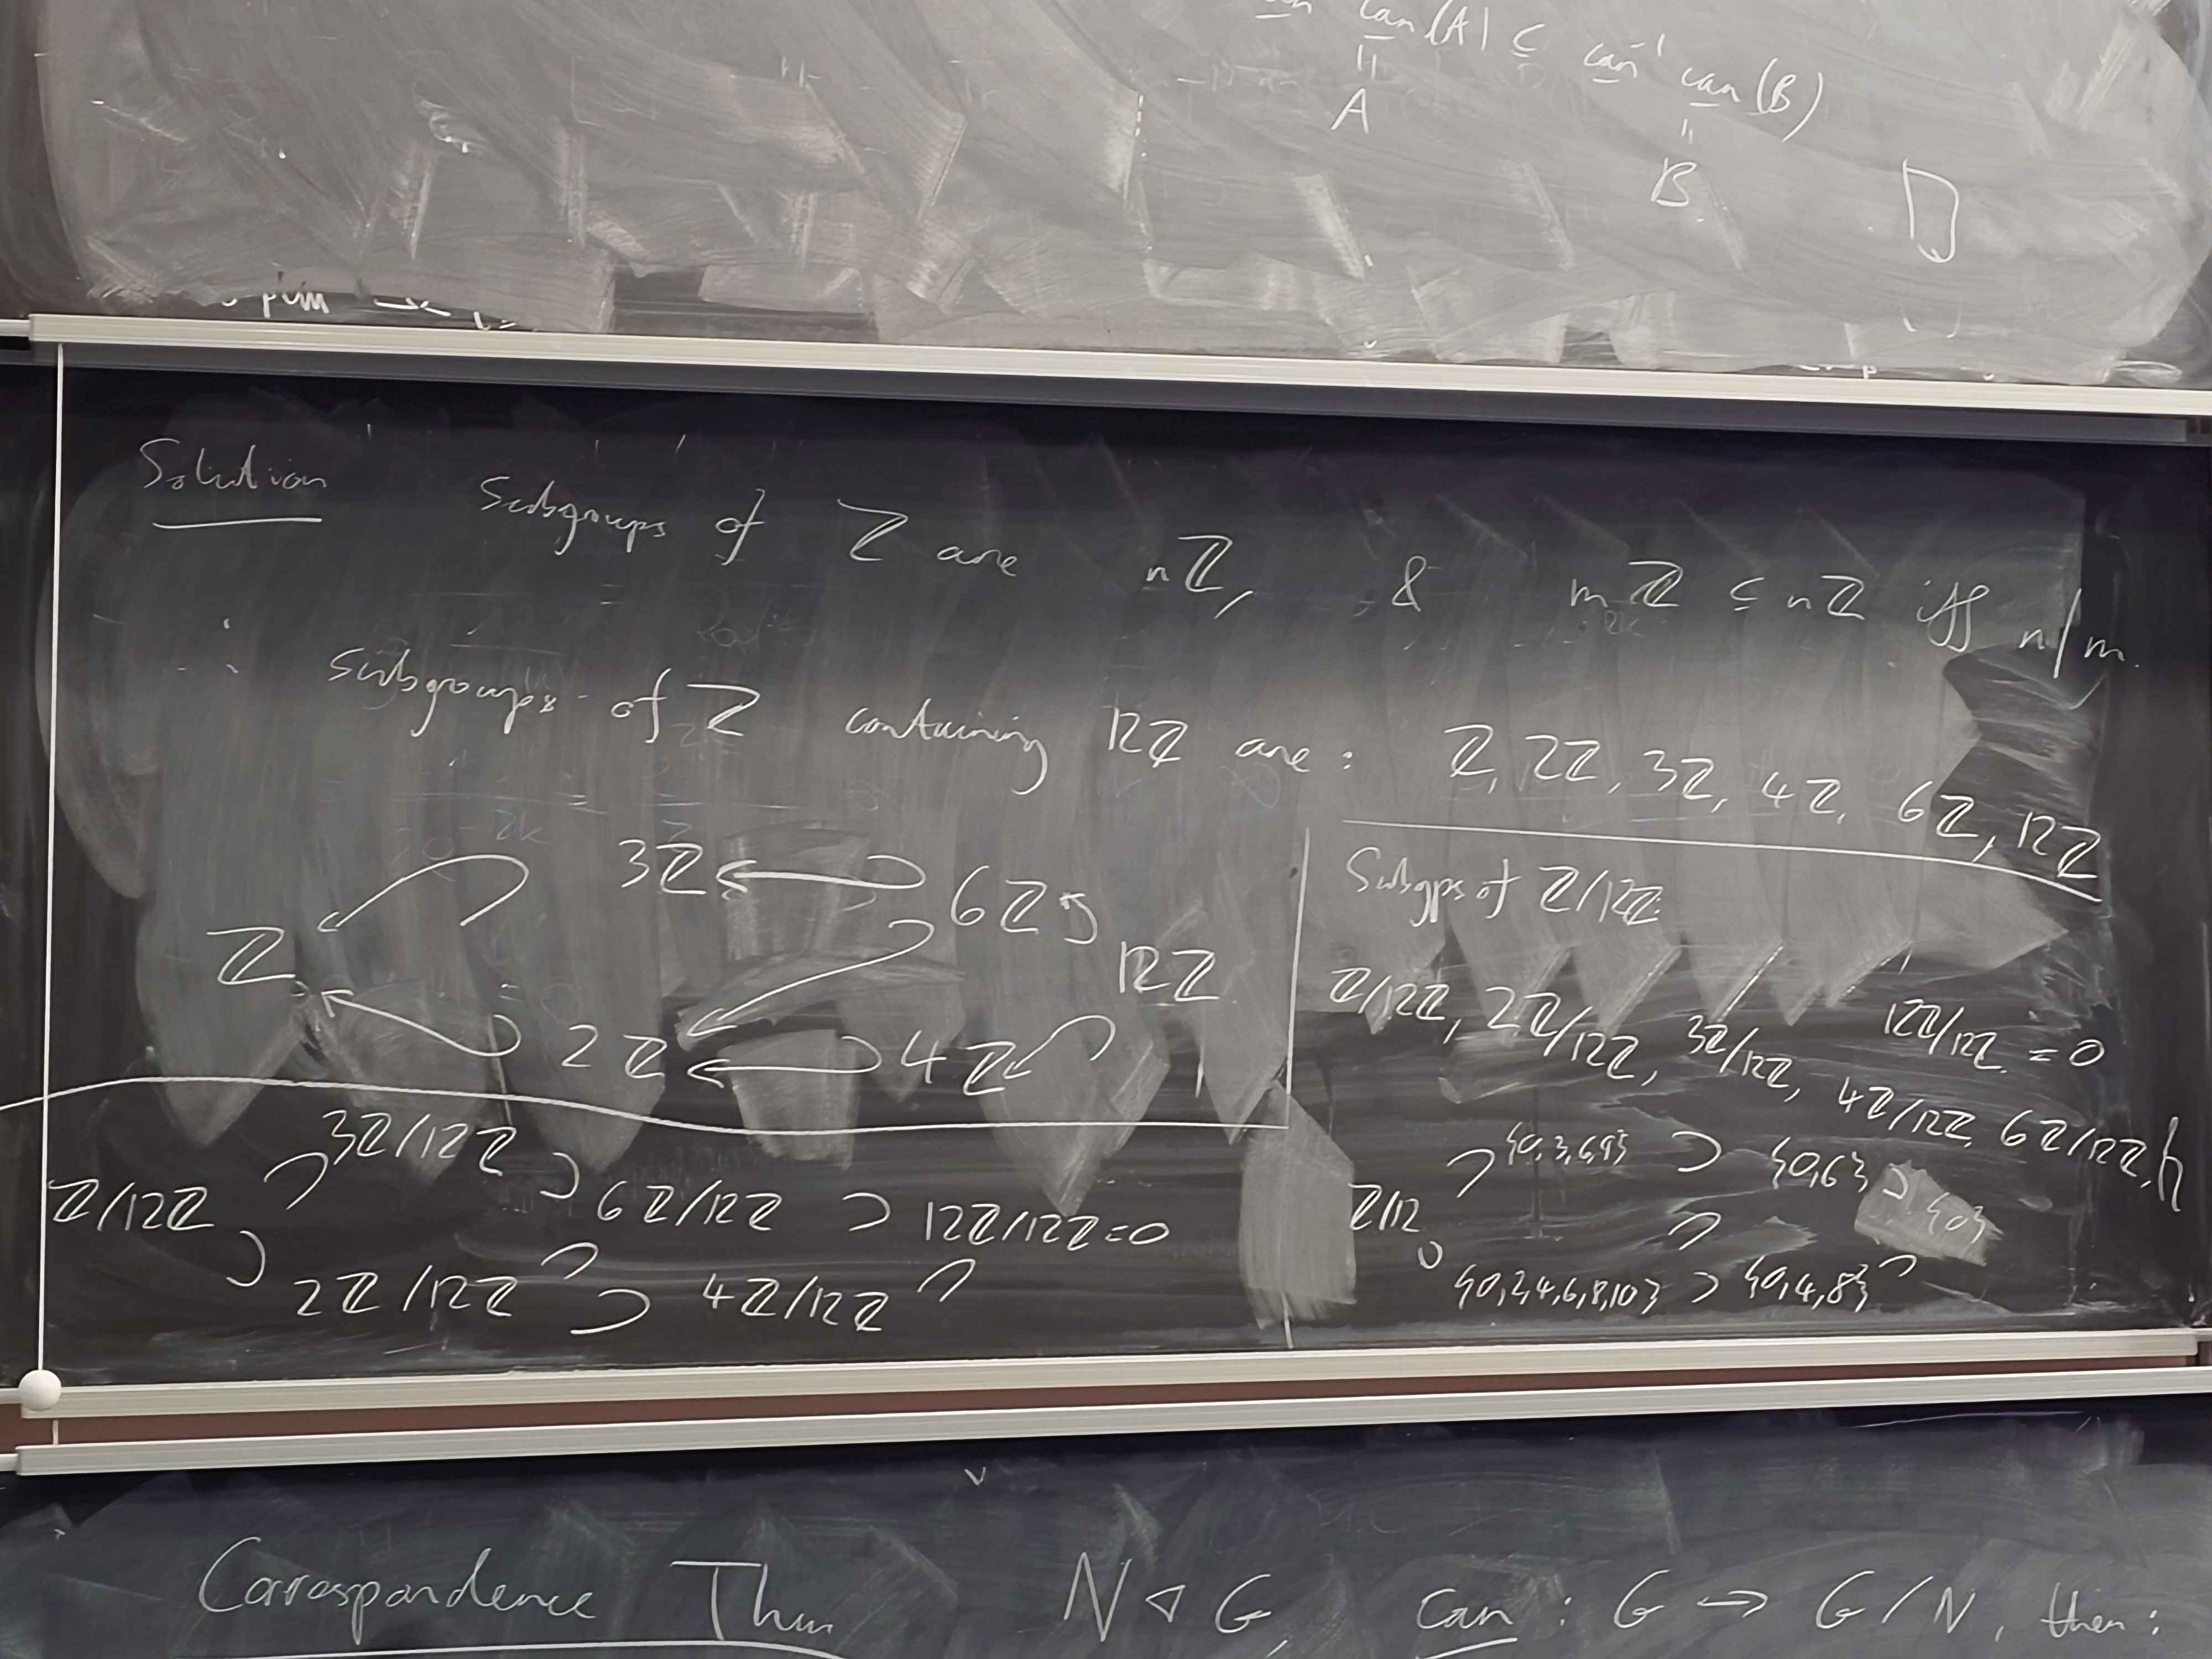
\includegraphics[width=\linewidth]{images/subgroup-diagram.jpg}
\end{figure}

\textbf{Subgroups of $\mathbb{Z} / 12\mathbb{Z}$}:
\[12\mathbb{Z} /12\mathbb{Z},\, \mathbb{Z} / 12\mathbb{Z},\,2\mathbb{Z} /12\mathbb{Z},\,3\mathbb{Z} /12\mathbb{Z},\,4\mathbb{Z} /12\mathbb{Z},\,6\mathbb{Z} /12\mathbb{Z}\]

some working out

\begin{thm}[Third Isomorphism Theorem]{thm:third-iso-thm}{}
    If $N, H \triangleleft G$, with $N \le H$, then
    \[(G /N) / (H /N) \cong G /H\]
\end{thm}

\end{document}
